\documentclass[a4paper]{article}

\usepackage[english]{babel}
\usepackage[utf8]{inputenc}
\usepackage{amsmath}
\usepackage{graphicx}
\usepackage[colorinlistoftodos]{todonotes}
\usepackage{amssymb}

\title{Mapeos conformes y aplicaciones}
\author{Lourdes Oros Barrón}

\begin{document}
\maketitle

Presentamos propiedades de las funciones del espacio complejo que preservan \'angulos, son las llamadas conformes, así como algunas aplicaciones a la física cl\'asica, esto en el contexto de las funciones de variable compleja. Una propiedad escencial para abordar el tipo de problemas que veremos es el hecho de que bajo una transformación conforme las funciones armónicas, $u$ tal que $\nabla ^{2}u=0$, se mapean a funciones armónicas.

\section{Definiciones y resultados}

Sean $X$ y $Y$ espacios vectoriales en $\mathbf{C}$ de dimensi\'on finita y $f:X \rightarrow Y$ la función compleja $f(z)=u(x,y)+iv(x,y).$ Suponga que el punto $(u_{0}, v_{0})$ es la imagen del punto $(x_{0}, y_{0}),$ y que además las curvas $C_{1}(x, y)$ y $C_{2}(x, y)$ se intersectan en $(x_{0}, y_{0})$ y tienen curvas imagen $K_{1}(u, v)$ y $K_{2}(u, v)$ respectivamente, las cuales se cortan en $(u_{0}, v_{0}).$ 

\textit{Definición} La transformación $f$ en el contexto anterior, es conforme si el ángulo entre $C_{1}(x, y)$ y $C_{2}(x, y)$ es igual tanto en dirección como en sentido al ángulo entre $K_{1}(u, v)$ y $K_{2}(u, v).$ Figura \ref{fig:mapconf}.\\

\begin{figure}
\centering
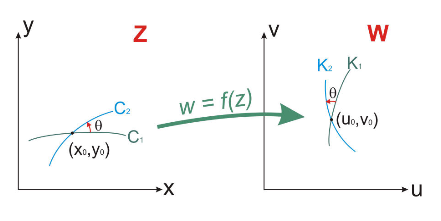
\includegraphics[width=0.7\textwidth]{mapconf.png}
\caption{\label{fig:mapconf} Mapeos conformes.}
\end{figure}

Formalmente, la función $f$ es conforme si existen números $r \in \mathbb{R}^{+}$ y $\theta \in [0, 2\pi)$ tales que:
\begin{itemize}
    \item Para cualquier curva diferenciable $\gamma : [0,1] \rightarrow \Omega,\, \gamma(0)=(x_{0}, y_{0})$ tenemos que $(f\circ  \gamma)'(0)|=r \dot |\gamma'(0)|$ y arg$(f\circ \gamma)'(0)=\theta +$ arg$(\gamma'(0)).$
    
    \item $f$ es conforme en cada punto de su dominio
\end{itemize}

\textbf{Teorema del mapeo conforme} Sean $\Omega \subset \mathbb{C}$ una región y $f: \Omega \rightarrow \mathbb{C}$ una función de clase $C^{1}$ en $\mathbb{R}^{2}$ y $z_{0} \in \Omega.$ La función $f$ es conforme en $z_{0}$ si y solo si $f$ es analítica y $f'(z_{0})\neq 0.$ \\
\textbf{Demostración:} Sean $A,B \subset \mathbb{C}$ y $f: A \rightarrow B$ y $\epsilon > 0.$ Supongamos que $f$ es conforme en $z_{0} \in A,$ de la hipótesis de que cada una de sus componentes es de clase $C^{1},$ para mostrar que $f$ es analítica será suficiente mostrar que satisface las ecuacioones de Cauchy-Riemann.\\
Consideremos la curva $\gamma : [0,\epsilon] \rightarrow \mathbb{C},$ dada por $\gamma(t)=z_{0}+t.$ Como $\gamma(0)=z_{0}$ y $$
(f \circ \gamma)(t)=u(x_{0}+t, y_{0})+iv(x_{0}+t, y_{0})$$ entonces $$(f \circ \gamma)'(0)=u_{x}(x_{0}, y_{0})+iv_{x}(x_{0}, y_{0})=f_{x}(x_{0}, y_{0}).$$\\
Consideremos ahora la curva $\delta :[0, \epsilon] \rightarrow \mathbb{C}$ como $\delta(t)=z_{0}+it,$ entonces $\delta(0)=z_{0}$ y un cálculo similar al anterior mostrará que:$$
(f \cdot \delta)'(0)=u_{y}(x_{0}, y_{0})+iv_{y}(x_{0}, y_{0})=f_{y}(x_{0}, y_{0}).$$
Luego, como $\gamma'(0)=1$ y $\delta'(0)=i$ entonces:
$|\gamma'(0)|=|\delta'(0)|$
y
$arg(\delta'(0))=\frac{\pi}{2}+arg(\gamma'(0)),$ asi $
\gamma'(0)=-i\delta'(0).
$\\
Las mismas relaciones geométricas se cumplen para $(f \circ \gamma)'(0)$ y $(f \circ \delta)'(0),$ con ello:
$$
f_{x}(x_{0},y_{0})=-if_{y}(x_{0},y_{0}).
$$ Asi, $f$ es diferenciable en el sentido complejo en $z_{0}.$ Finalmente, $f'(z_{0}) \neq 0$ pues de la definición de conformidad, el factor $r > 0$ y con ello $f'(z_{0})\neq 0.$

Recíprocamente, supongamos que $f$ es real-diferenciable en $z_{0}$ y que $f'(z_{0}) \neq 0.$ Sea $r=|f'(z_{0})| \geq 0$ y sea $\eta=arg(f'(z_{0})).$ Entonces para cualquier curva diferenciable $\phi,$ con $\phi(0)=z_{0},$ de la regla de la cadena, se tendrá que $$
(f \circ \phi)'(0)=f'(z_{0}) \phi'(z_{0})
$$
y con ello $$
|(f \circ \phi)'(0)|=|f'(z_{0})||\phi'(0)|=r|\phi'(0)|
$$ y $$
arg((f \circ \phi)'(0))=arg(f'(z_{0}))+arg(\phi'(0))= \theta +
arg(\phi'(0)).
$$\\

\textbf{Teorema de representación conforme}\\
Dado un conjunto $D \subset \mathbb{C}$ abierto y simplemente conexo, existe una transformación conforme, $f,$ tal que $f(D)$ es el disco abierto unitario.\\

\textit{Algunos ejemplos sencillos son los siguientes:}\\
\textit{Rotación.} $z \mapsto ze^{i\frac{\pi}{4}}$. Si $z=e^{i\theta}$ con $\theta \in [0, 2\pi)$ y $f(z)=ze^{i\frac{\pi}{4}}$ entonces $f'(z)=e^{i\frac{\pi}{4}} \neq 0$ $\forall z$, por lo que $f$ es conforme. Ver \ref{fig:fun2}.\\
\begin{figure}
\centering
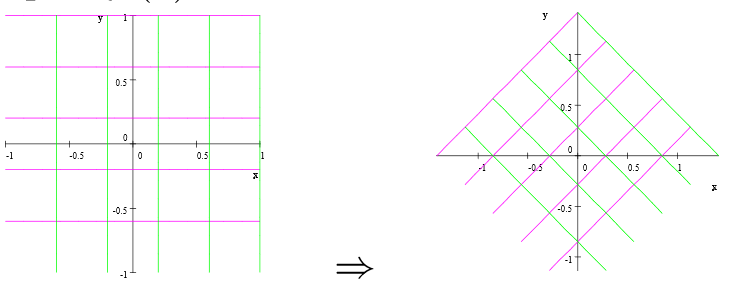
\includegraphics[width=0.7\textwidth]{fun2.png}
\caption{\label{fig:fun2} Función $f(z)=ze^{i\frac{\pi}{4}}$.}
\end{figure}

\textit{Inversión}: $f(z)=\frac{1}{z}$ Transforma el conjunto formado por todas las rectas y circunferencias en él mismo.. Se tiene que $f'(z)=\frac{-1}{z^{2}}\neq 0$ $\forall z \neq 0,$ entonces el mapeo es conforme. Ver \ref{fig:fun1}.\\
\begin{figure}
\centering
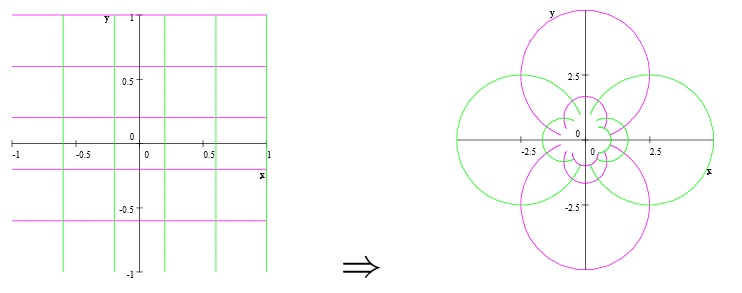
\includegraphics[width=0.7\textwidth]{fun1.jpg}
\caption{\label{fig:fun1} Función $f(z)=\frac{1}{z}$}
\end{figure}

Veremos ahora uno de los ejemplos más importantes en variable compleja:\\
Una transformación fraccional lineal (también llamada transformación de Möbius) es una transformación de la forma $$
T(z)=\frac{az+b}{cz+d} 
$$ donde $a,b,c$ y $d$ son números complejos fijos. Supondremos que $ad-bc \neq 0$ pues en este caso $T$ sería constante.\\

\textbf{Proposición.}
La transformación $T$ definida anteriormente es biyectiva y conforme del conjunto $$
A=\{z|cz+d \neq 0 , esto es, z \neq \frac{-d}{c}\}
$$ sobre el conjunto $B=\{w|w \neq \frac{a}{c}\}.$
Más aún $
T^{-1}(w)=\frac{-dw+b}{cw-a}.$\\
\textbf{Demostración.}
T es claramente analítica en $A$ y $S(w)=\frac{-dw+b}{cw-a}$ es analítica en $B.$ Para demostrar la biyectividad basta demostrar que $T\circ S$ y $S \circ T$ son la identidad. En efecto pues:$$
T(S(w))=\frac{a(\frac{-dw+b}{cw-a})+b}{c(\frac{-dw+b}{cw-a})+d}
=\frac{-adw+ab+bcw-ab}{-cdw+bc+dcw-da}
=\frac{bc-ad}{bc-ad}w=w.
$$ Análogamente $S(T(z))=z.$\\
Finalmente $T'(z)\neq 0$ pues $$
\frac{d}{dz}S(T(z))=\frac{d}{dz}z=1
$$ y así $$
S'(T(z)) \cdot T'(z) \neq 0.
$$ Por lo tanto $T'(z) \neq 0$ y con ello, es una transformación conforme.\\
La importancia de este ejemplo yace en el estudio de variable compleja.
Vista en el plano complejo, $T$ es la composición de una proyección estereográfica del plano sobre la esfera, seguida de una rotación o desplazamiento de la esfera a una nueva localización y finalmente una proyección estereográfica, esta vez de la esfera al plano.\\

\section{Aplicaciones de los mapeos conformes}
%\subsection{La ecuación de Laplace}
%En cálculo vectorial, la \textit{ecuación de Laplace} es una ecuación de derivadas parciales de segundo orden.\\
%\textbf{Definición:} En dos dimensiones, el problema consiste en hallar funciones reales dos veces diferenciables $u$ de variables reales $x,y$ tal que: $$
%\frac{\partial^2 u}{\partial x^{2}}+\frac{\partial^2 u}{\partial y^{2}}+=0.$$
%Las soluciones a esta ecuación de denominan funciones armónicas, todas analíticas dentro del dominio donde la ecuación es válida.
%Aparece en ramas de la física teórica como astronomía, electrostática, mecánica de fluidos y mecánica cuántica.
%La ecuación así planteada, no tiene solución única, sin embargo, cuando se estableces condiciones de contorno o condiciones iniciales se tiene únicidad en la solución.\\
%Los problemas de este tipo se pueden resolver usando técnicas de variable compleja denominados \textit{Problema de Dirichet} y \textit{Problema de Newmann}.\\

\subsection{Problema de Dirichlet}
Consiste en encontrar una función $u(x,y)$ con dominio $D,$ dos veces diferenciable tal que $\nabla ^{2} U(x,y)=0$ para todo $(x,y)\in D.$ Bajo la condición de que $\frac{\partial u}{\partial \eta}=0$ para todo $(x,y) \in Fr(D).$ Donde $\eta$ es el vector normal a la curva que define la frontera de $D,$ y por lo tanto $\frac{\partial u}{\partial \eta}$ es la derivada direccional del campo $u$ en la dirección de ese vector normal.
 
\subsection{Problema de Newmann}
Consiste en encontrar una función $u(x,y)$ con dominio $D,$ dos veces diferenciable tal que $\nabla ^{2} U(x,y)=0$ para todo $(x,y)\in D.$ Bajo la condición de que $u(x,y)=u_{0}$ para todo $(x,y) \in Fr(D).$\\

Cuando el dominio $D$ es simplemente conexo sabemos, por el teorema de la representación conforme , que es posible hallar una función analítica $f$ con derivada no nula tal que  la transformación de $D$ por esta función sea otro dominio simplemente conexo $D'.$\\
\textbf{¿En qué problema se transforman tanto el de Dirichlet como el de Newmann cuando cambiamos el dominio con una transformación conforme?}

La respuesta a esta cuestión nos la dan las siguientes proposiciones, las cuales indican que un problema de Dirichlet se va a transformar en uno de Dirichlet, lo mismo para el problema de Newmann.\\

\textbf{Proposiciones:}\\
\begin{itemize}
\item Sea $G(x,y)$ una función armónica en un dominio $D$ simplemente conexo y $f(x,y)=u(x,y)+iv(x,y)$ una transformación conforme en $D,$ llamemos $D'=f(D).$ Entonces la función $g(u,v)=G(x(u,v), y(u,v))$ es también una función conforme en $D'.$
\item Si $G(x,y)=G_{0}$ es una función constante, entonces $g(u,v)$ es la mkisma función constante.
\item Si $\frac{\partial G}{\partial \eta}=0$ en la frontera de $D'$ y si $N$ es el vector normal a la curva transformada por la función conforme es $\frac{\partial g}{\partial N}=0.$
\end{itemize}

De lo anterior podemos concluir que si $f$ es una transformación conforme tal que $f(D)=D'$ con $D$ simplemente conexo y si $g(u,v)$ es la transformada de $G(x,y)$ mediante $f$ entonces el problema de Dirichlet se transforma en otro de Dirichlet de la forma:$$
\frac{\partial ^{2}g}{\partial u^{2}}+\frac{\partial ^{2}g}{\partial v^{2}}=0
$$ para todo $(u,v)\in D'$ con la condición $g(u,v)=G_{0}$ para todo $(u,v) \in Fr(D').$

\subsection{Conducción del calor}
Para un problema de transferencia de calor, las curvas de nivel de una función armónica corresponden a las llamadas isotermas, y una derivada normal igual a cero corresponde al aislamiento térmico. Para ilustrar estas ideas, consideramos el problema simple de transferencia de calor en estado estacionario. Se muestra el esquema en la figura \ref{fig:res}.\\
Se tiene una tubería cilíndrica con cavidad cilíndrica no centrada por la que pasa el vapor a $100^{\circ} C$. La temperatura exterior de la tubería es de $0^{\circ} C$. El radio del círculo interior es $\frac{3}{10}$ del radio de círculo exterior, así que si elegimos el radio exterior como unidad de longitud, el problema puede ser formulado 
como el de encontrar una función armónica $T(u, v)$ tal que$$
\frac{\partial ^{2}T}{\partial x^{2}} + \frac{\partial ^{2}T}{\partial y^{2}} = 0 $$ en la región entre los círculos $|z|=1$ y $|z-0.3|=0.3,$ y $T=0$ sobre $|z|=1$ y $T=100$ sobre $|z-0.3|=0.3.$

\begin{figure}
\centering
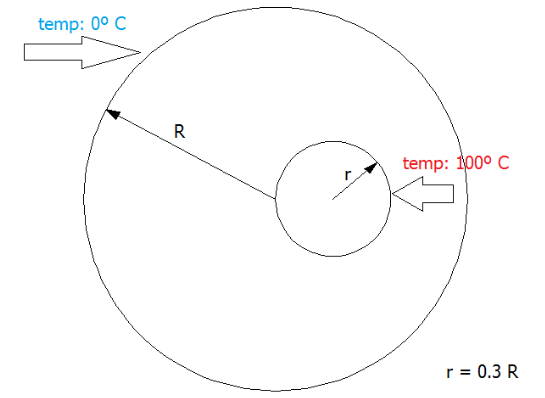
\includegraphics[width=0.3\textwidth]{res.png}
\caption{\label{fig:res} Diagrama esquemático del problema de transferencia de calor}
\end{figure}

La función $z \mapsto \frac{z-3}{3z-1}$ transforma el círculo $|z|=1$ en el circulo $|w|=1$ y el circulo $|z-0.3|=0.3$ en el circulo $|w|=3.$

Asi el problema se convierte en uno de simetria del plano $w$ que consiste en encontrar una función armónica $T(u,v)=100$ en $|w|=1$ y $T(u,v)=0$ en $|w|=3.$\\
Las funciones armónicas con tal simetris son de la forma: $$
T(u,v)=A\ln(u^{2}+v^{2})+B
$$ donde $A$ y $B$ son constantes.\\
Asi, para nuestro caso, si $T(u,v)=100$ en $u^{2}+v^{2}=1$ y $T(u,v)=0$ en $u^{2}+v^{2}=9.$ Asi $B=100$ y $A=-100 \ln(9),$ por lo que la solucipon en el plano $w$ es $$
T(u,v)=\frac{100 \ln[1-\ln(u^{2}+v^{2})]}{\ln(9).}
$$ Ver \ref{fig:res}.
Necesitamos la solución en el plano $z,$ es decir, tenemos que obtener $u$ y $v$ en términos de $x$ y de $y.$ Y como $u^{2}+v^{2}=|w^{2}|$ y $$
|w^{2}|=|\frac{z-3}{3z-1}|^{2}
=\frac{|z-3|^{2}}{|3z-1|^{2}}
=\frac{(x-3)^{2}+y^{2}}{(3x-1)^{2}+9y^{2}}.
$$
\begin{figure}
\centering
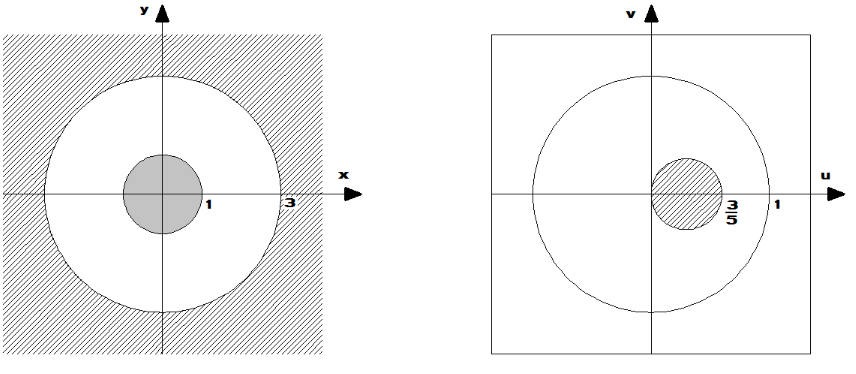
\includegraphics[width=0.7\textwidth]{fig4.png}
\caption{\label{fig:fig2} $z\mapsto \frac{z-3}{3z-1}$.}
\end{figure}

Finalmente, la solución es:$$
T(x,y)=\frac{100}{\ln(9)} {1-\ln[(x-3)^{2}+y^{2}]-\ln[(3x-1)^{2}+9y^{2}]}.
$$. Ver \ref{fig:fig2}. \\

\subsection{Potencial eléctrico}
De la física sabemos que si un potencial eléctrico $\phi$ está determinada por cargas eléctricas estáticas entonces debe satisfacer la ecuación de Laplace (que es la condición de ser armónica). La función conjugada $\Phi$ de $\phi$ se interpreta como sigue: Las líneas a lo largo de las cuales $\Phi$ es constante, son lineas a través de las cuales viajará una pequeña carga, estas son llamadas líneas de flujo. Los vectores tangentes a tales líneas son $-\nabla \phi=E,$ llamado el campo eléctrico. Así las líneas de flujo y las lineas donde $\phi$ es constante (llamadas equipotenciales) se intersectan ortogonalmente. Ver \ref{fig:electrico}.\\

\begin{figure}
\centering
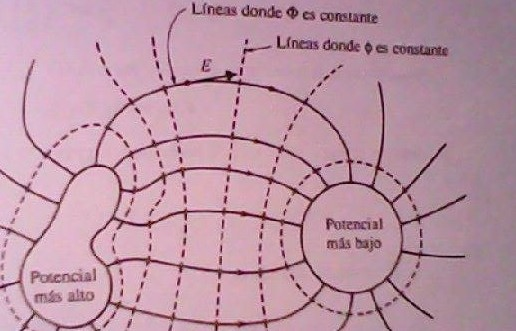
\includegraphics[width=0.7\textwidth]{electrico.jpg}
\caption{\label{fig:electrico} Potencial eléctrico.}
\end{figure}

\textbf{Ejemplo.} Considere el círulo unitario. El potencial eléctrico es mantenido en $\phi=0$ en el semicirculo inferior y en $\phi=1$ en el semicírculo superior. Encuentre la $\phi$ superior.\\
\textit{Solución:} Transformando la región dada en el semiplano superior a tavés de la transformación conforme: $$
z \mapsto \frac{1}{i} \frac{z-1}{z+1}
$$ que es la usada para resolver el problema de Dirichlet en el disco.
Como la temperatura es físicamente razonable que el potencial esté acotado. Ver \ref{fig:Dirichlet}.\\\\
\begin{figure}
\centering
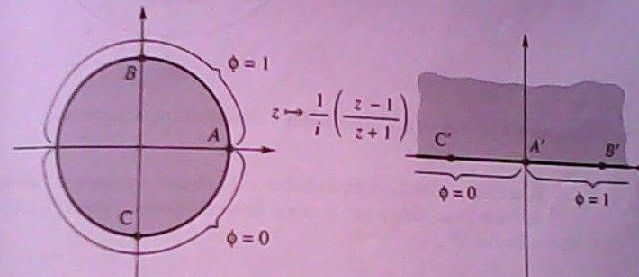
\includegraphics[width=0.7\textwidth]{Dirichlet.jpg}
\caption{\label{fig:Dirichlet} Mapeo conforme para resolver el problema de Dirichlet en el disco.}
\end{figure}

Asi, la solución es $$
\phi_{0}(x,y)=1-\frac{1}{\pi}tan^{-1}(\frac{y}{x})
$$ y por lo tanto la solución en el círculo unitario es:
$$
\phi(x_{0}, y_{0})=\phi_{0}(f(x, y))
$$ donde $f(z)=\frac{1}{i} \frac{z-1}{z+1}.$ Visto en $\mathbb{R}^{2}$ la solución es:$$
\phi(x,y)=1-\frac{1}{\pi} \tan^{-1}(\frac{1-x^{2}-y^{2}}{2y}).
$$
El problema de Dirichlet surge en electrostática cuando la frontera se mantiene en un potencial dado(haciendo tierra o por medio de una bateria).\\

\section{Conclusiones}
La idea general de usar mapeos conformes sobre funciones armónicas es la siguiente:
\begin{itemize}
\item Buscar una función conforme que transforme el dominio donde esté definido el problema al circulo unitario o al semiplano $Im z \geq 0.$
\item Usar métodos conocidos para resolver el problema transformado.
\item Emplear la inversa de la función $f$ para encontrar la solución del problema original.
\end{itemize}

\section{Bibliografía}
\begin{enumerate}    
\item
“Variable Compleja, Transformaciones Conformes”, M. Eugenia Torres, Universidad de Entre Ríos, Facultad de Ingeniería
\item
Análisis básico de variable compleja, Jerrold E. MArsden, Michael J. Hoffman.
\item
Notas. "Aplicaciones de propiedades de funciones armónicas y transformaciones conformes", Pesce, Javier Alfonso.
\end{enumerate}
\end{document}